\section{Appendix}

\FloatBarrier

Supplements to simulation study (experiment 2)

\begin{figure}
	\centering
	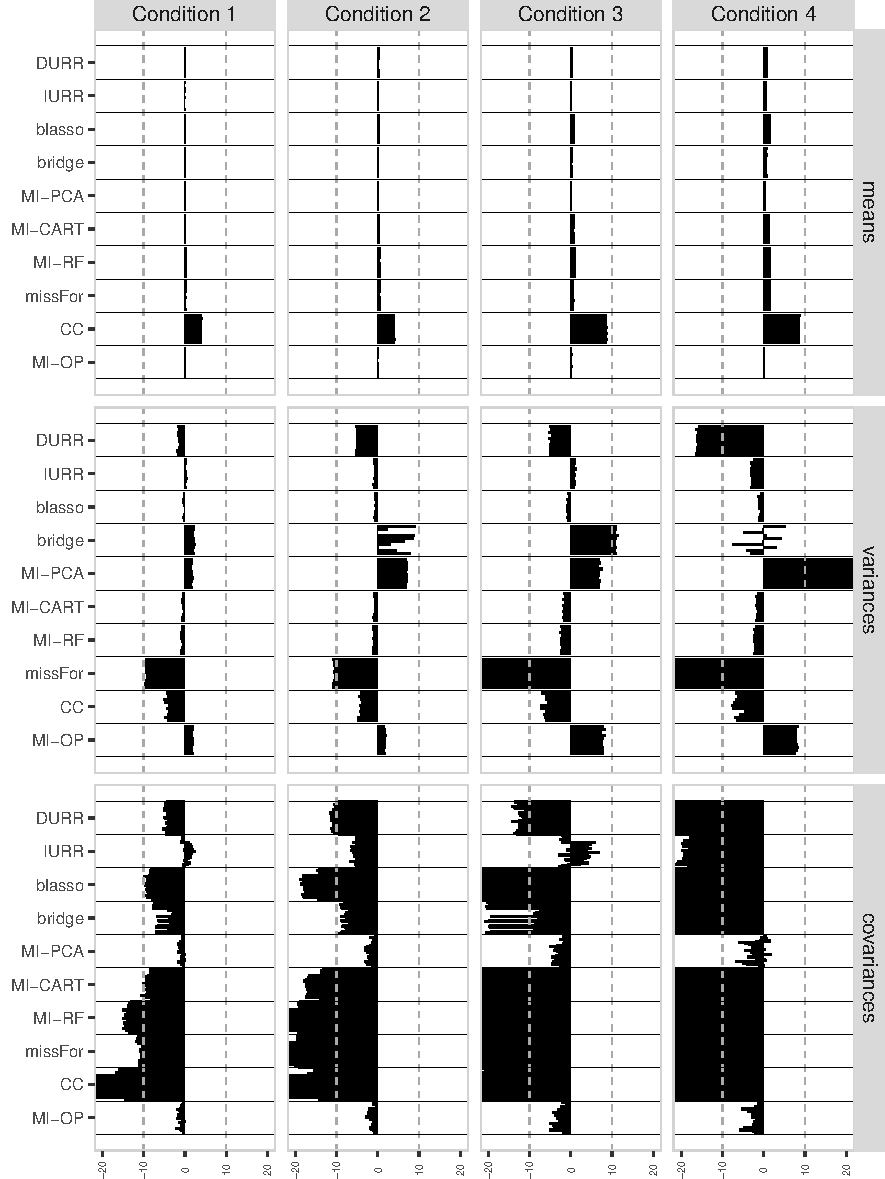
\includegraphics{\pathFIG/exp2_semR_bias_58.pdf}
	\caption{Bias estimation for the means (SB), variances and covariances (PRB) for condition 5 
			to 8.}
	\label{fig:exp2bias58}
\end{figure}

\begin{figure}
	\centering
	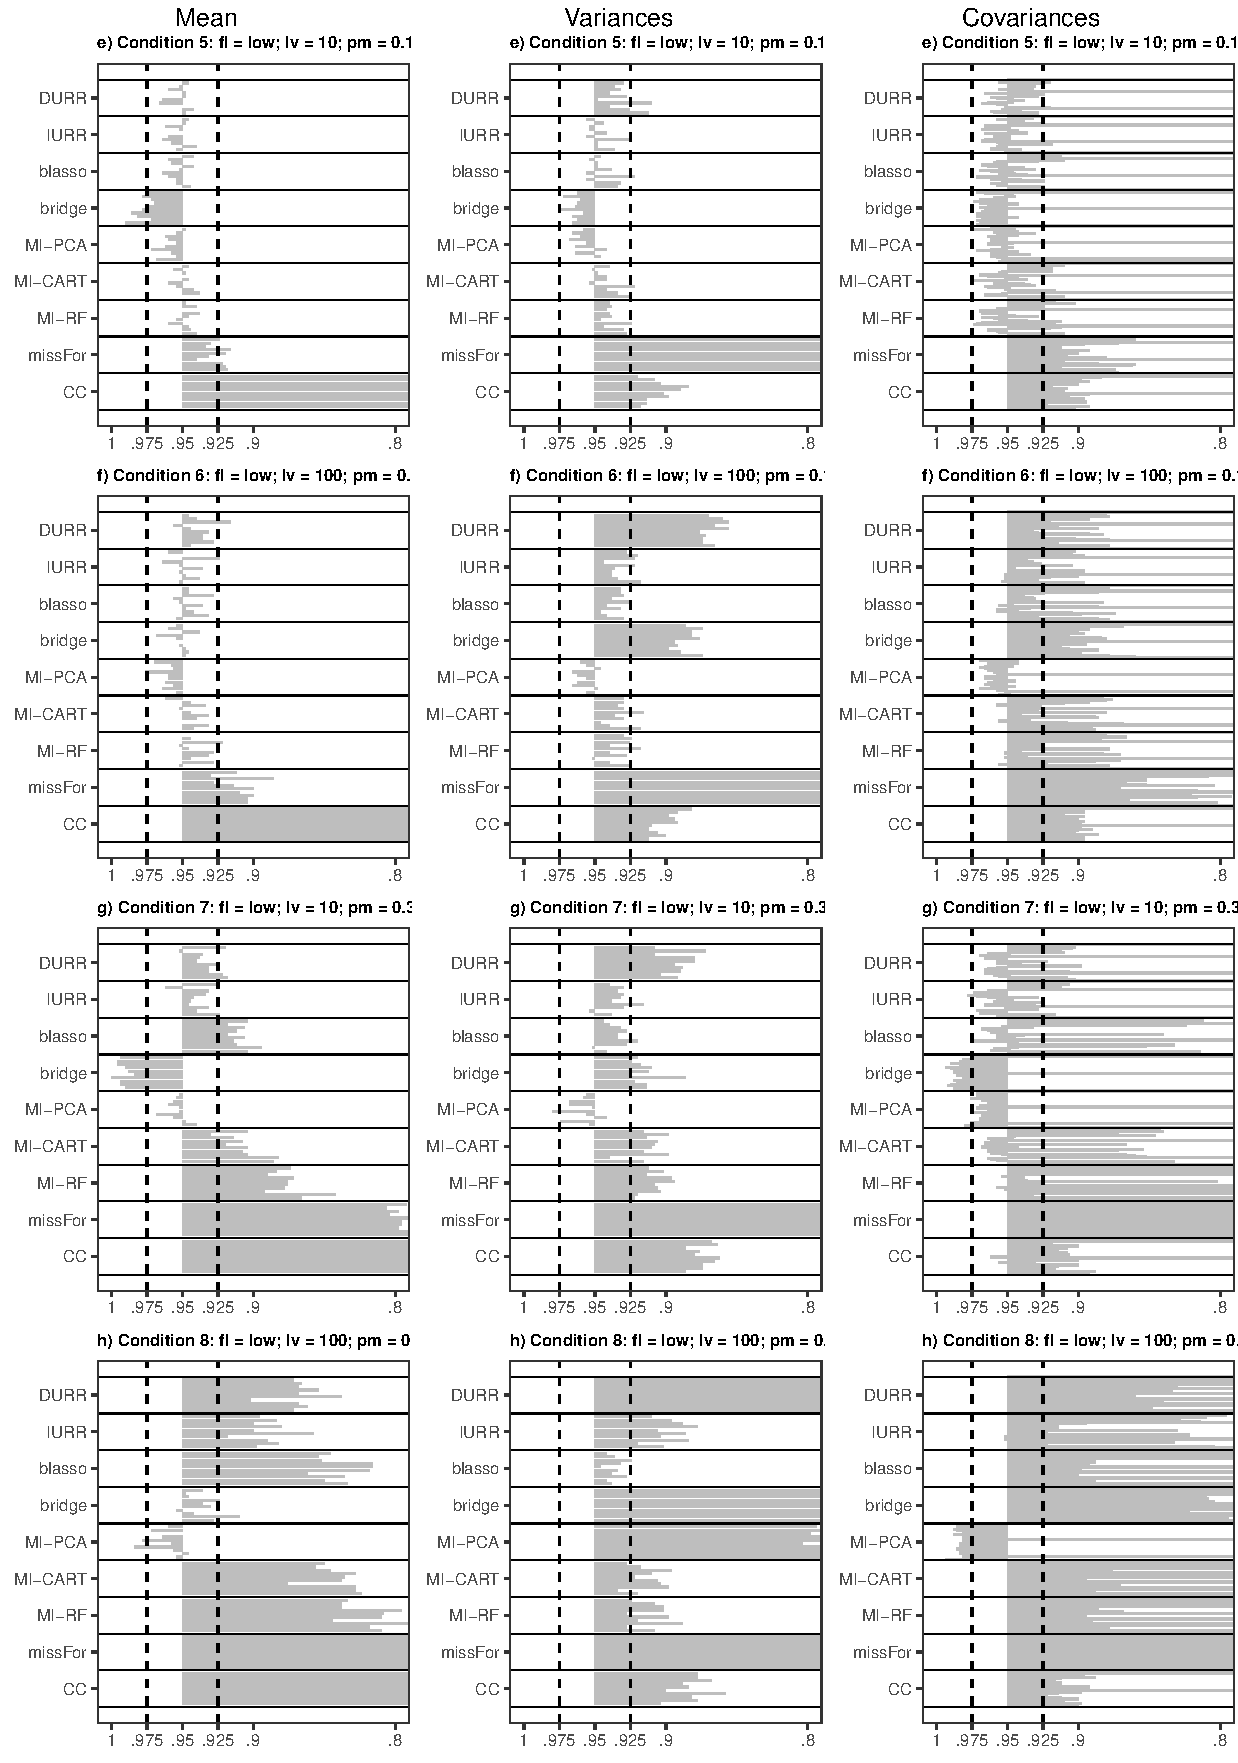
\includegraphics{\pathFIG/exp2_semR_ci_58.pdf}
	\caption{Confidence Interval Coverage (CIC) for the means, variances, and covariances 
			for condition 5 to 8.}
	\label{fig:exp2cir58}
\end{figure}

Supplements to resampling study

\begin{figure}
	\centering
	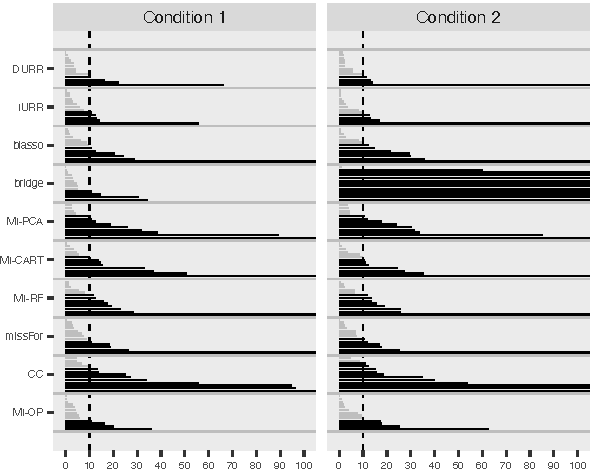
\includegraphics{\pathFIG/exp4_imp_bias_allParms_m1.pdf}
	\caption{PRBs for all the model parameters in model 1. 
		The order of the bars is based on the absolute value of the PRBs.
		The values for the intercept, the focal regression coefficient, and the regression coefficient with which most 
		methods struggle (Largest Bias) are highlighted}
	\label{fig:exp4bias_m1}
\end{figure}

\begin{figure}
	\centering
	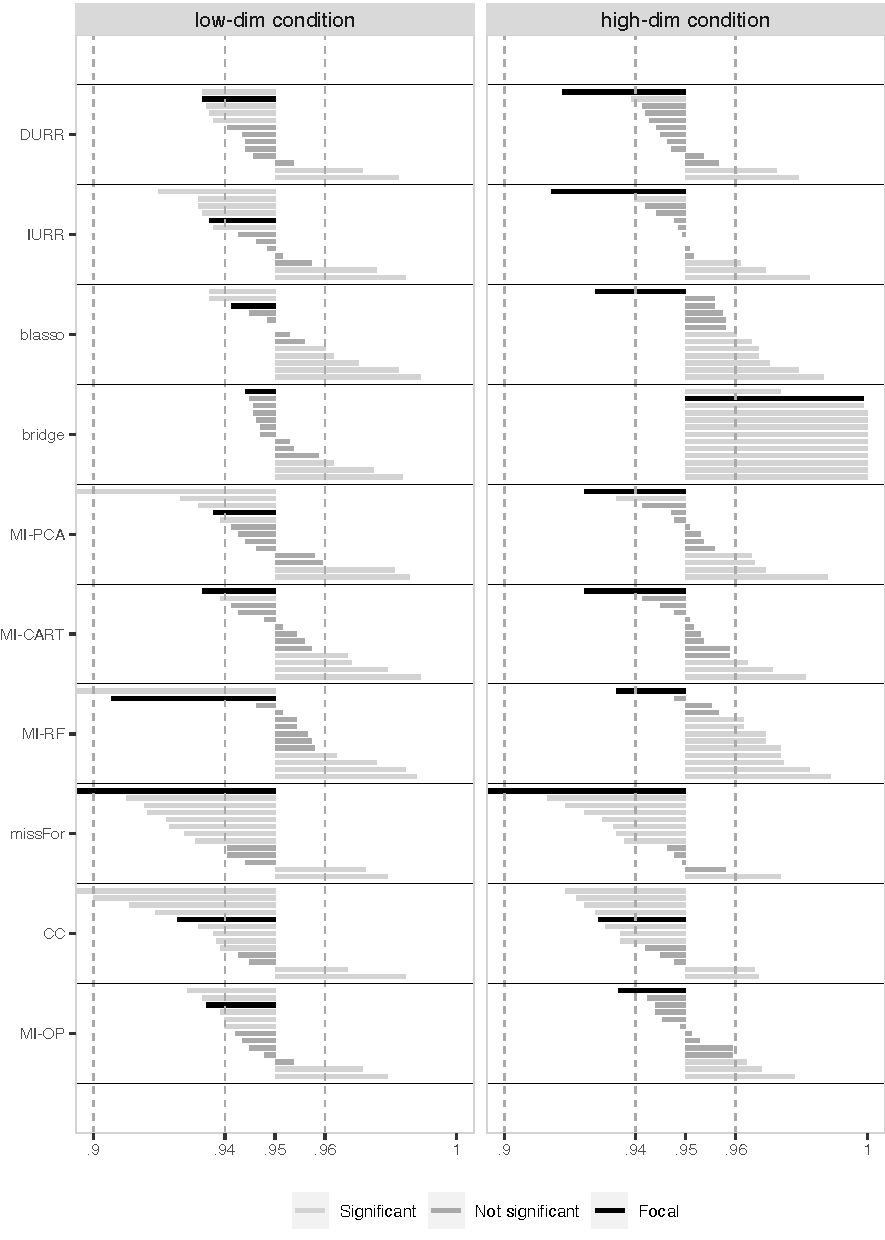
\includegraphics{\pathFIG/exp4_imp_ci_allParms_m1.pdf}
	\caption{CIC for all model parameter in model 1.
		Bars are sorted in by ascending value.
		The values for the intercept, the focal regression coefficient, and the regression coefficient with which most 
		methods struggle (Largest Bias) are highlighted}
	\label{fig:exp4cir_m1}
\end{figure}

\FloatBarrier
